%------------------------- ADDITIONAL MATERIAL -------------------------%
\section{Additional Material} \label{app:additional_material}

No detailed additional literature review material was required for the creation of the concepts.

%------------------------- DECISION ANALYSIS TABLES -------------------------%
\section{Decision Analysis Tables} \label{app:decision_analysis_tables}

Decision analysis' are shown in the following tables. Concepts are scored (S) from 1 (worst) to 3 (best). This is then multiplied by the weight to get the weighed score (WS) and a total sum is calculated for each solution. The concept with the highest total is the winner.

Table \ref{table:decision_analysis_robot} shows the decision analysis for the robot locomotion concepts. 
The highest weight of 30/100 is attributed to power consumption, as the solution must be solar powered, making power a limiting factor. The scores are attributed based on the number of electric motors on each solution. 

The next criteria, weighed at 20/100, is mobility and terrain operation. This includes ability to turn, navigate on slopes and walk in various difficult terrains such as sand, pebbles, shallow water, mud and small plants. 

The next criteria weighs 20/100 as well and consists of feasibility and design complexity. This relates to the the simplicity of the design as well as the complexities that may arise in further analysis of the design (force concentrations on parts, number of components to consider, etc). 

Furthermore, maintainability and longevity is added with a weight of 15/100. This is included due to the fact that the robot should be self-reliant. It takes into account frequency and ease of maintenance.

The last two criteria are: aesthetics (10/100) as the robot operates in public areas, and cost (5/100) which is a minor consideration due to the fact that this solution has very little existing competition. It is still considered in order to ensure the designs' feasibility. 


\begin{table}[H]
    \centering
    \caption{Decision analysis table for robot and leg concepts}
    \label{table:decision_analysis_robot}
    \begin{tabular}{ | p{3.5cm} | >{\centering\arraybackslash}p{1.5cm} | >{\centering\arraybackslash}p{1cm} | >{\centering\arraybackslash}p{1cm} | >{\centering\arraybackslash}p{1cm}| >{\centering\arraybackslash}p{1cm} | >{\centering\arraybackslash}p{1cm} | >{\centering\arraybackslash}p{1cm}|}
        \hline
        Criteria & Weight & \multicolumn{2}{c|}{Concept 1} & \multicolumn{2}{c|}{Concept 2} & \multicolumn{2}{c|}{Concept 3}
        \\ \hline
         &  & S & WS & S & WS & S & WS
        \\ \hline
        Power Consumption & 30 & 3 & 90 & 2 & 60 & 1 & 30
        \\ \hline
        Mobility and Terrain Operation & 20 & 1 & 20 & 2 & 40 & 3 & 60
        \\ \hline
        Feasibility and Design Complexity & 20 & 1 & 20 & 3 & 60 & 2 & 40
        \\ \hline
        Maintainability and Longevity & 15 & 3 & 45 & 1 & 15 & 2 & 30
        \\ \hline
        Aesthetics & 10 & 1 & 10 & 2 & 20 & 3 & 30
        \\ \hline
        Cost & 5 & 3 & 15 & 2 & 10 & 1 & 5
        \\ \hline
        Total & 100 &  & 200 &  & 205 &  & 195
        \\ \hline
    \end{tabular}
\end{table}

Table \ref{table:decision_analysis_solar} shows the decision analysis for the solar panel solutions. 

The most critical criteria, weighed at 35/100 is to maximise the sun exposure surface. This includes maximising the surface area of the solar panels as well as orienting them in a favourable manner towards the sun. It determines the amount of power output from the solar panels. 

The second highest weighed criteria, with 30/100, is compatibility and integration. This includes whether the solar panels could impede with the movement of the robots' legs or other moving parts. It also takes into account whether it could potentially interfere with the integration of the waste collecting system designed by group 2B. It was discussed that a garbage container might be positioned on top of the robot, with an arm moving to deposit waste in the container.

Stability, weighed at 20/100, takes into account the effects of the solar panels on the center of mass of he robot and whether they could get caught in the wind. Lastly, cost is included as a measure of complexity of the solutions, and weighs 15/100.

\begin{table}[H]
    \centering
    \caption{Decision analysis table for solar panel concepts}
    \label{table:decision_analysis_solar}
    \begin{tabular}{ | p{3.5cm} | >{\centering\arraybackslash}p{1.5cm} | >{\centering\arraybackslash}p{1cm} | >{\centering\arraybackslash}p{1cm} | >{\centering\arraybackslash}p{1cm}| >{\centering\arraybackslash}p{1cm} | >{\centering\arraybackslash}p{1cm} | >{\centering\arraybackslash}p{1cm}|}
       \hline
        Criteria & Weight & \multicolumn{2}{c|}{Concept 1} & \multicolumn{2}{c|}{Concept 2} & \multicolumn{2}{c|}{Concept 3}
        \\ \hline
         &  & S & WS & S & WS & S & WS
        \\ \hline
        Maximise Sun Exposed Surface Area & 35 & 3 & 105 & 1 & 35 & 2 & 70
        \\ \hline
        Cost & 15 & 1 & 15 & 2 & 30 & 3 & 45
        \\ \hline
        Compatibility and Integration & 30 & 2 & 60 & 1 & 30 & 3 & 90
        \\ \hline
        Stability & 20 & 1 & 20 & 2 & 40 & 3 & 60
        \\ \hline
        Total & 100 &  & 200 &  & 135 &  & 265
           \\ \hline
    \end{tabular}
\end{table}



%------------------------- DETAILED COST ASSESSMENT-------------------------%
\section{Detailed Cost Assessment} \label{app:cost_assessment}
The references to all sources used in the cost assessment tables can be found in Table \ref{table:source_reference}.
The quote for Harmonic Drives provided by Electromate was given in CAD; this number was converted to USD for a fair comparison with other expensive components such as motors and gearboxes.

\begin{table}[H]
    \centering
  \caption{Cost Analysis for Concept 1 - Linkage}
  \label{table:cost_linkage}
  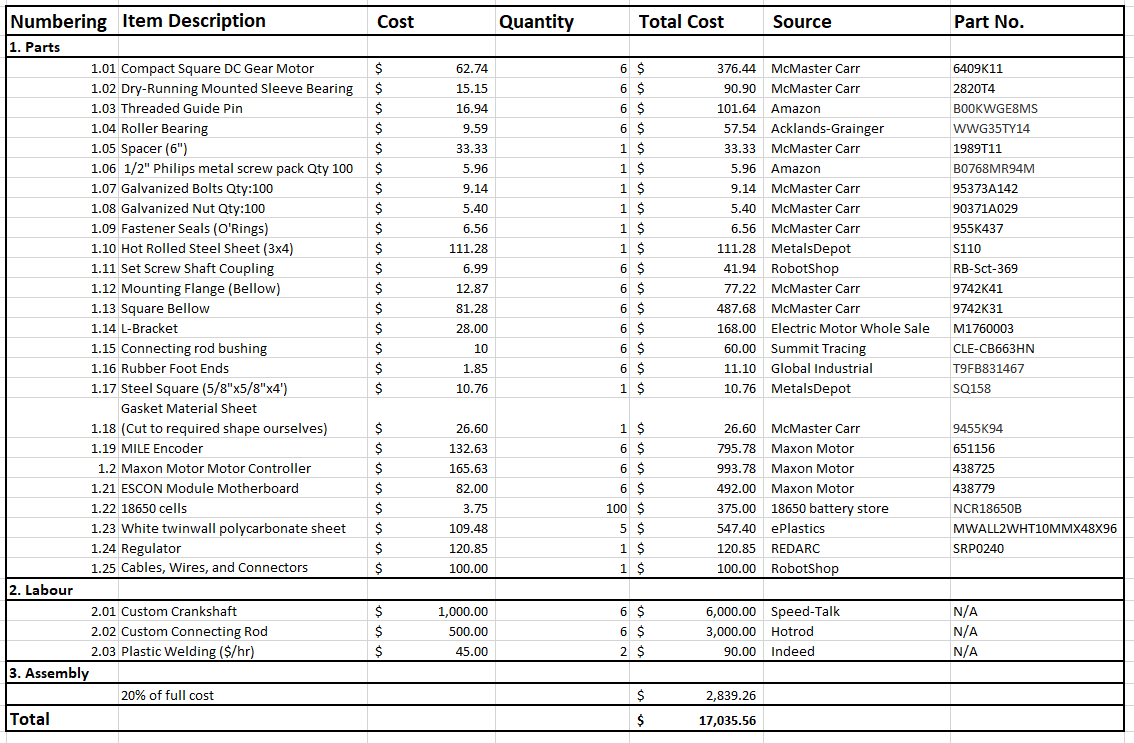
\includegraphics[width=0.9\linewidth]{Cost/C1.PNG}
\end{table}

\begin{table}[H]
  \caption{Cost Analysis for Concept 2 - Crab}
  \label{table:cost_crab}
  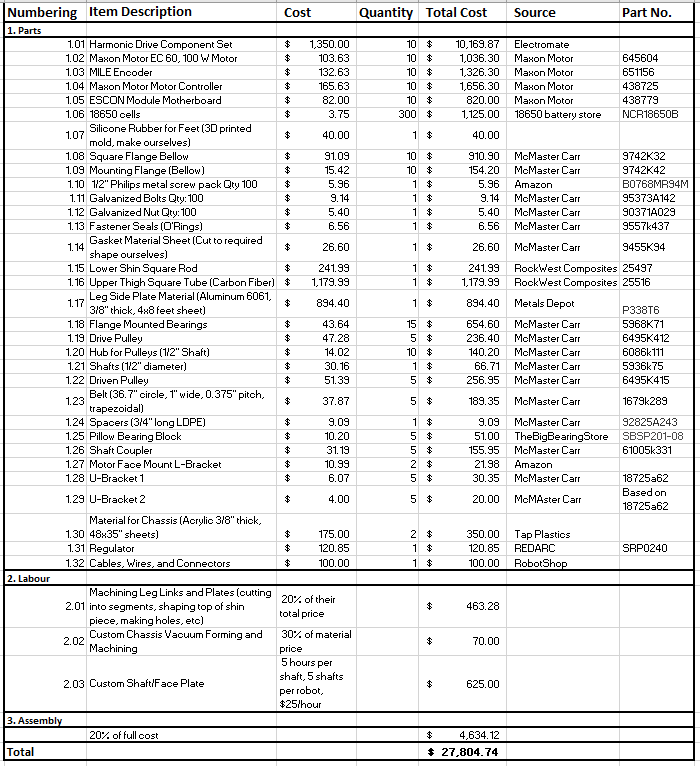
\includegraphics[width=\linewidth]{Cost/C2.PNG}
\end{table}

\begin{table}[H]
  \caption{Cost Analysis for Concept 3 - Spider}
  \label{table:cost_spider}
  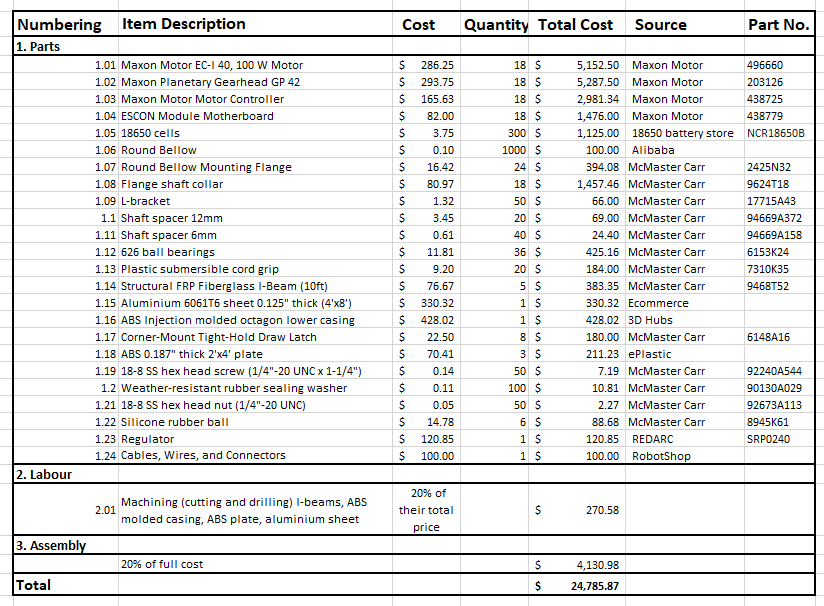
\includegraphics[width=\linewidth]{Cost/C3.PNG}
\end{table}

\begin{table}[H]
  \caption{Cost Analysis for Solar Concept 1 - Roof}
  \label{table:cost_solar_roof}
  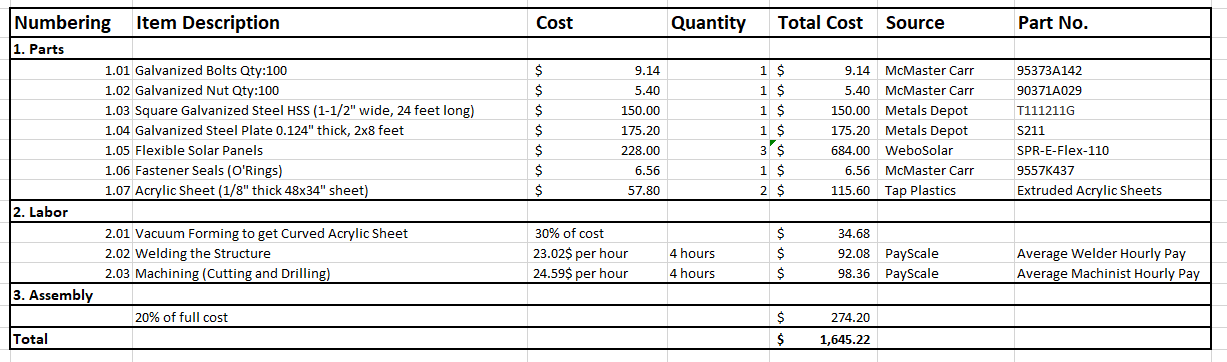
\includegraphics[width=\linewidth]{Cost/S1.PNG}
\end{table}

\begin{table}[H]
  \caption{Cost Analysis for Solar Concept 2 - Awning}
  \label{table:cost_solar_awning}
  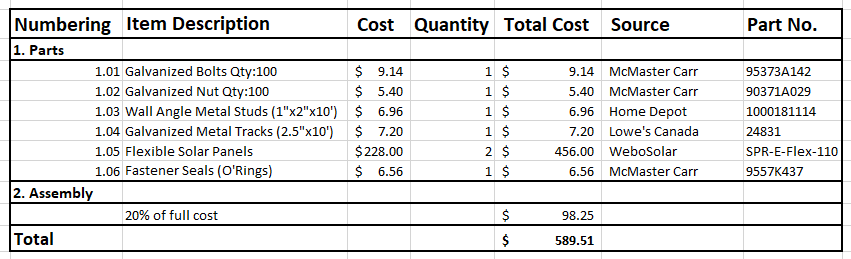
\includegraphics[width=\linewidth]{Cost/S2.PNG}
\end{table}

\begin{table}[H]
  \caption{Cost Analysis for Solar Concept 3 - Solar Cells}
  \label{table:cost_solar_cells}
  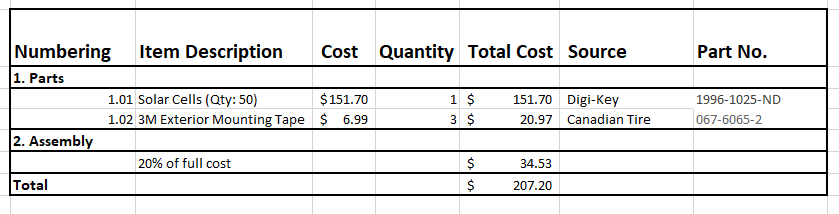
\includegraphics[width=\linewidth]{Cost/S3.PNG}
\end{table}

\begin{center}
    \begin{longtable}{ l c }
        \caption{Part Source References}
        \label{table:source_reference}
         \\ \hline
          3D Hubs & \cite{3d_hubs_3d_nodate}
         \\ \hline
         18650 battery store & \cite{18650_battery_store_18650_nodate}
         \\
         Acklands-Grainger & \cite{acklands-grainger_acklands-grainger_nodate}
         \\ \hline
         Alibaba & \cite{alibaba_alibaba_nodate} 
         \\ \hline
         Amazon & \cite{amazon_amazon_nodate} 
         \\ \hline
         Canadian Tire & \cite{canadian_tire_canadian_nodate} 
         \\ \hline
         DigiKey & \cite{digikey_digikey_nodate} 
         \\ \hline
         Electric Motor Wholesale & \cite{electric_motor_wholesale_electric_nodate} 
         \\ \hline
         Electromate & \cite{electromate_electromate_nodate} 
         \\ \hline
         ePlastics & \cite{eplastics_eplastics_nodate} 
         \\ \hline
         Speed-Talk & \cite{speed-talk_finding_nodate} 
         \\ \hline
         Global Industrial Canada & \cite{global_industrial_canada_global_nodate} 
         \\ \hline
         Home Depot & \cite{home_depot_home_nodate} 
         \\ \hline
         Hot Rod Network & \cite{hot_rod_network_hot_nodate} 
         \\ \hline
         Indeed & \cite{indeed_indeed_nodate} 
         \\ \hline
         Lowe's Canada & \cite{lowes_canada_lowes_nodate} 
         \\ \hline
         Maxon Motor & \cite{maxon_motor_maxon_nodate} 
         \\ \hline
         McMaster-Carr & \cite{mcmaster-carr_mcmaster-carr_nodate}
         \\ \hline
         Metal Supermarkets & \cite{metal_supermarkets_metal_nodate} 
         \\ \hline
         Metals Depot & \cite{metals_depot_metals_nodate}
         \\ \hline
         PayScale & \cite{payscale_payscale_nodate}
         \\ \hline
         REDARC & \cite{redarc_electronics_redarc_nodate}
         \\ \hline
         RobotShop & \cite{robots_shop_robotshop_nodate} 
         \\ \hline
         Rock West Composites & \cite{rock_west_composites_rock_nodate} 
         \\ \hline
         Summit Racing & \cite{summit_racing_summit_nodate} 
         \\ \hline
         TAP Plastics & \cite{tap_plastics_tap_nodate} 
         \\ \hline
         The Big Bearing Store & \cite{the_big_bearing_store_big_nodate} 
         \\ \hline
         Webo Solar & \cite{webo_solar_webo_nodate} 
         \\ \hline
    \end{longtable}
\end{center}

\subsection{Battery Selection}

Batteries were selected in the following manner:

\begin{enumerate}
    \item Power consumption per motor was set at 50W; not all motors will be running at the same time, nor at full capacity, so 50\% of total capacity was selected.
    \item Power consumption for computers is set conservatively to the full power of NVIDIA Jetson TX2s; these consume more power than Raspberry Pis and Arduinos, giving a conservative approximation \cite{gadget_makers_blog_arduino_2013} \cite{raspi.tv_how_2019} \cite{nvidia_jetson_2018}.
    \item The battery voltage matches the highest voltage element in the robot. This is likely the motors, which in the given configuration need 24 V, compared to up to 15 V for the NVIDIA Jetson TX2 \cite{nvidia_jetson_2018} \cite{maxon_motor_ec60_nodate}.
    \item A runtime of two hours was selected. This is in line with the two to four hours advertised by ANYbotics' ANYmal and hour-and-a-half advertised by Boston Dynamics' Spot \cite{anybotics_anymal_nodate} \cite{boston_dynamics_spot_2019}.
    \item The  Panasonic NCR18650B variant of 18650 cell were selected (same model as used in Tesla batteries), with 3.6 V and 3400mAh (12.58 Wh) \cite{18650_battery_store_18650_nodate} \cite{lambert_tear_2016}.
    \item The number of cells required is equal to the number of cells required to achieve the desired voltage, times the number of cells required to achieve the two hour runtime. In the case of the crab model, it requires seven cells in series and 42 is parallel, or approximately 300 cells in total.
\end{enumerate}

\begin{center}
    \begin{longtable}{ c c c c }
        \caption{Approximate Power consumption of Crab Model (see Figure \ref{fig:crab_top}) (does not include losses)}
        \label{table:power_consumption}
         \\ \hline
          Device Name & Power Consumption (W) & No. of device & Total power consumption (W)
         \\ \hline
         Computer & 7.5 & 2 & 15
         \\
         DC Motor & 50 & 10 & 500
         \\ \hline
         Total & & & 530
         \\ \hline
    \end{longtable}
\end{center}

%------------------------- DATA SHEETS -------------------------%
\section{Data Sheets} \label{app:data_sheets}

Table \ref{table:data_sheets} contains references for all data sheets beyond this point.

\begin{center}
    \begin{longtable}{ l c c }
        \caption{Part Source References}
        \label{table:data_sheets}
         \\ \hline
        Item & Source & Part Number (if applicable)
        \\ \hline
        Harmonic Drive CSD & \cite{harmonic_drive_csd-2a_nodate} & N/A
        \\ \hline
        Maxon Motor GP42C & \cite{maxon_motor_maxon_nodate} & 203126
        \\ \hline
        Maxon Motor EC 60 & \cite{maxon_motor_ec60_nodate} & 645604
        \\ \hline
        Maxon Motor ECi 40 & \cite{maxon_motor_maxon_nodate} & 496660
        \\ \hline
        Panasonic 18650 Cell & \cite{panasonic_industrial_devices_specifications_nodate} & NCR18650B
        \\ \hline
        RockWest Composites Carbon Fibre & \cite{rock_west_composites_rock_nodate} & 25516
         \\ \hline
         McMaster-Carr DC Gearmotor & \cite{mcmaster-carr_mcmaster-carr_nodate} & 6409K11
         \\ \hline
    \end{longtable}
\end{center}

% UN-COMMENT THESE IN THE END
%\begin{comment}
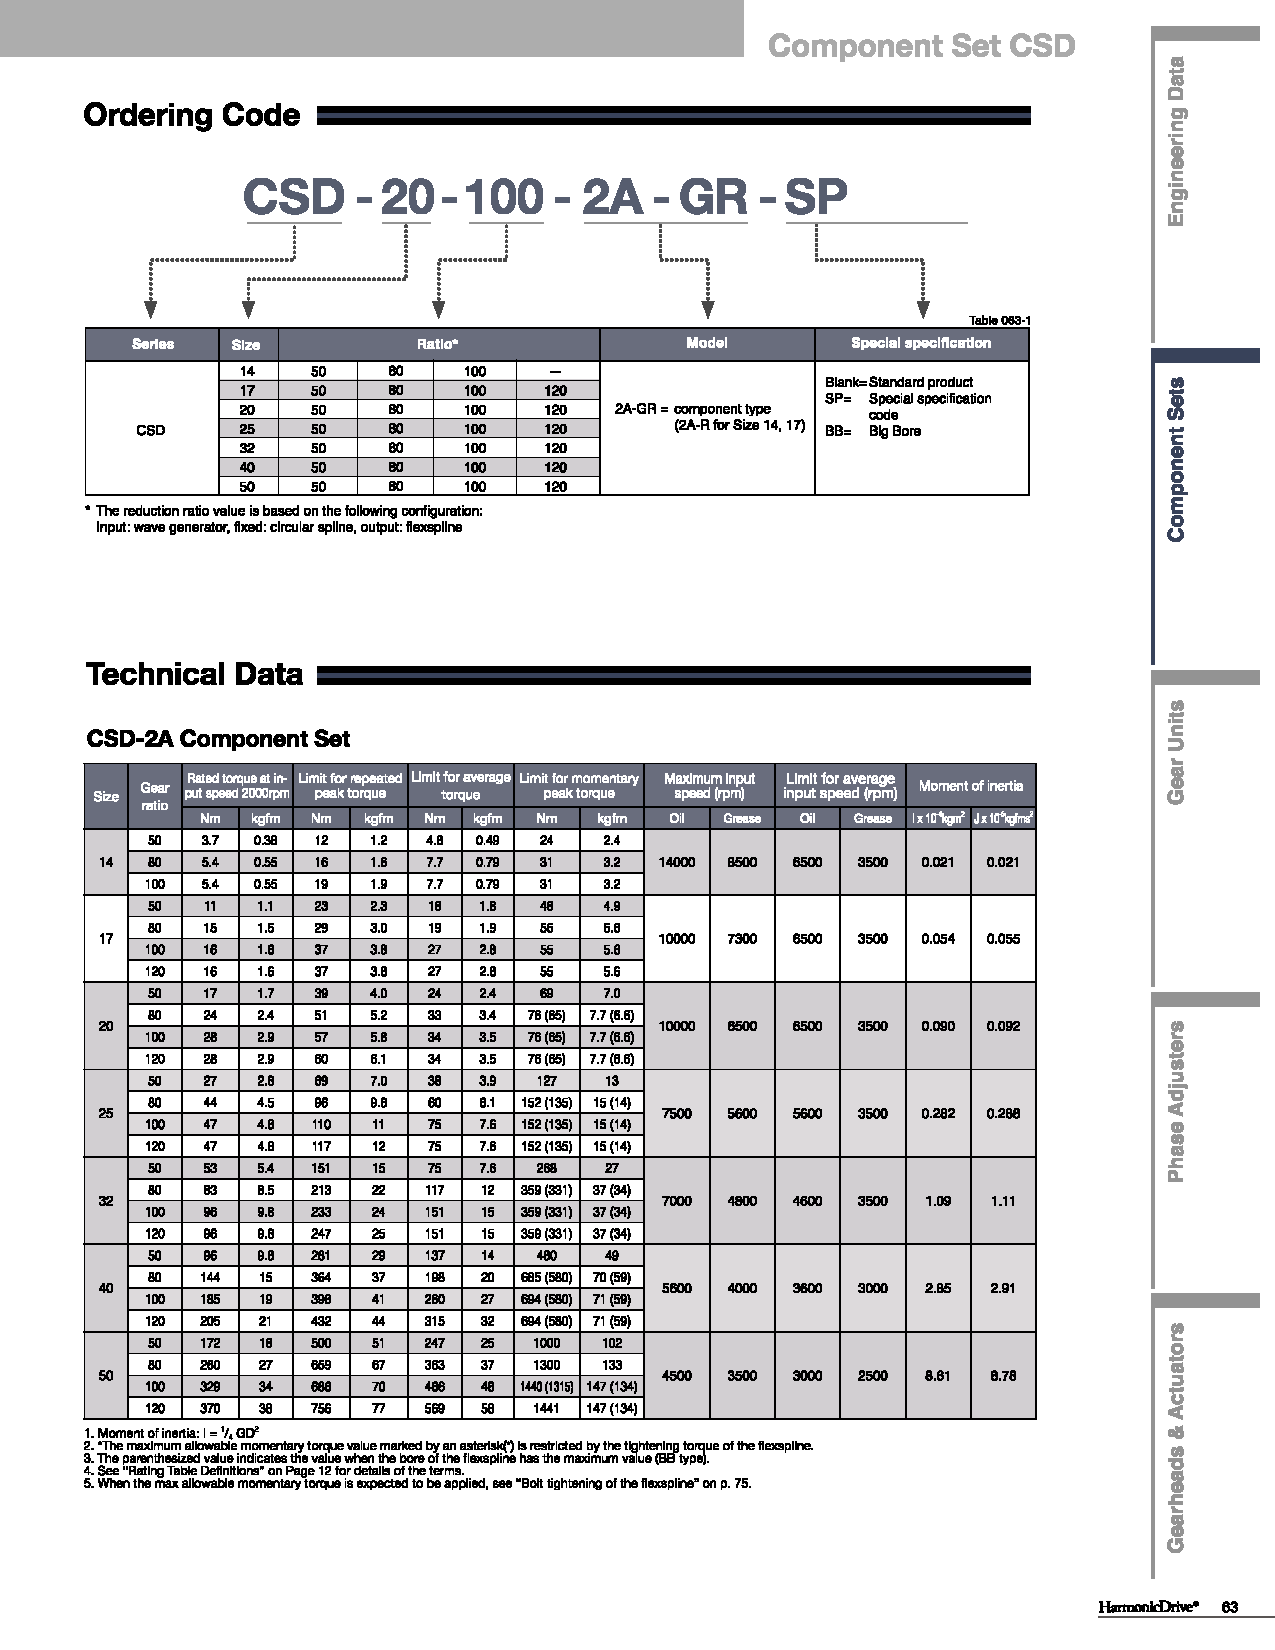
\includepdf[pages=-]{pdf/harmonic_drive_csd}
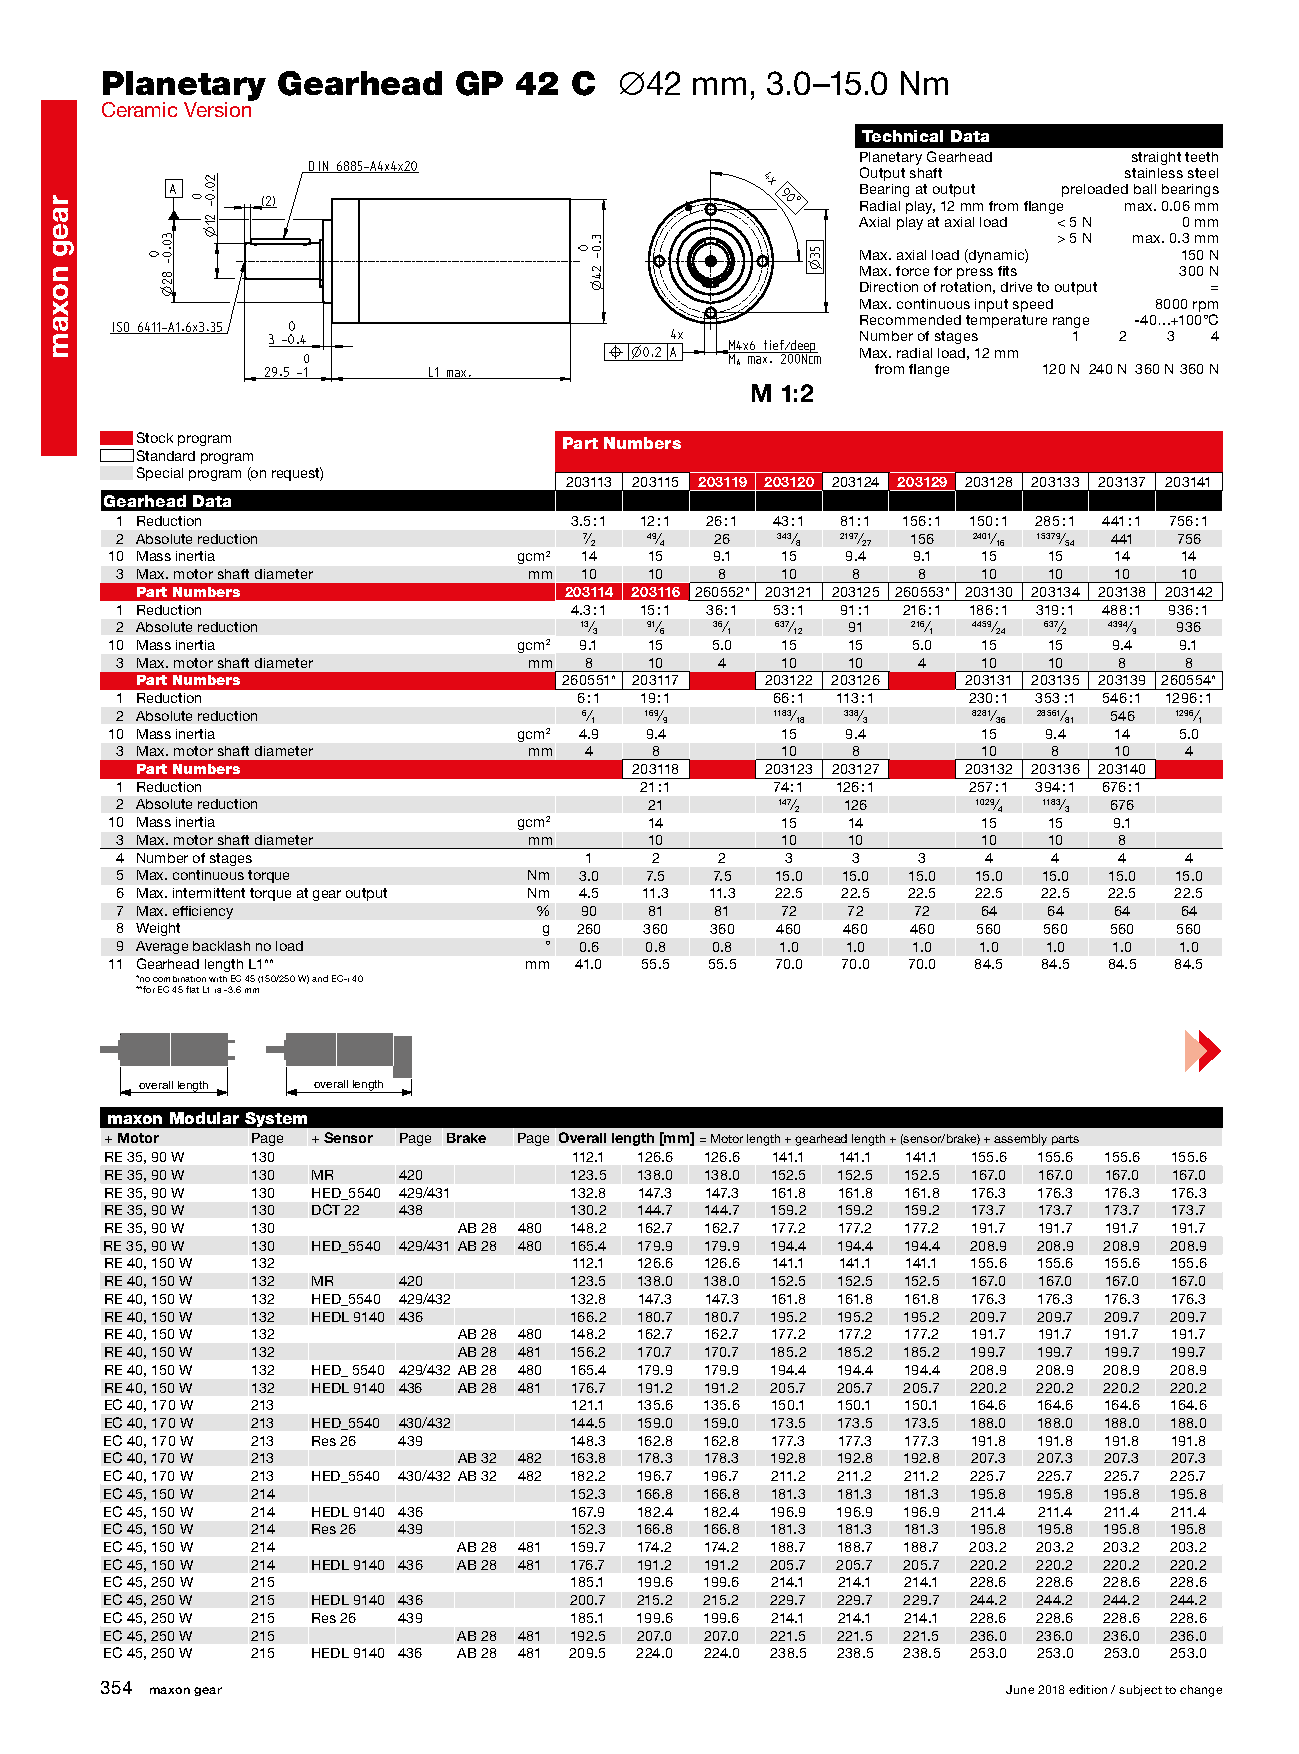
\includepdf[pages=-]{pdf/maxon_GP42C}
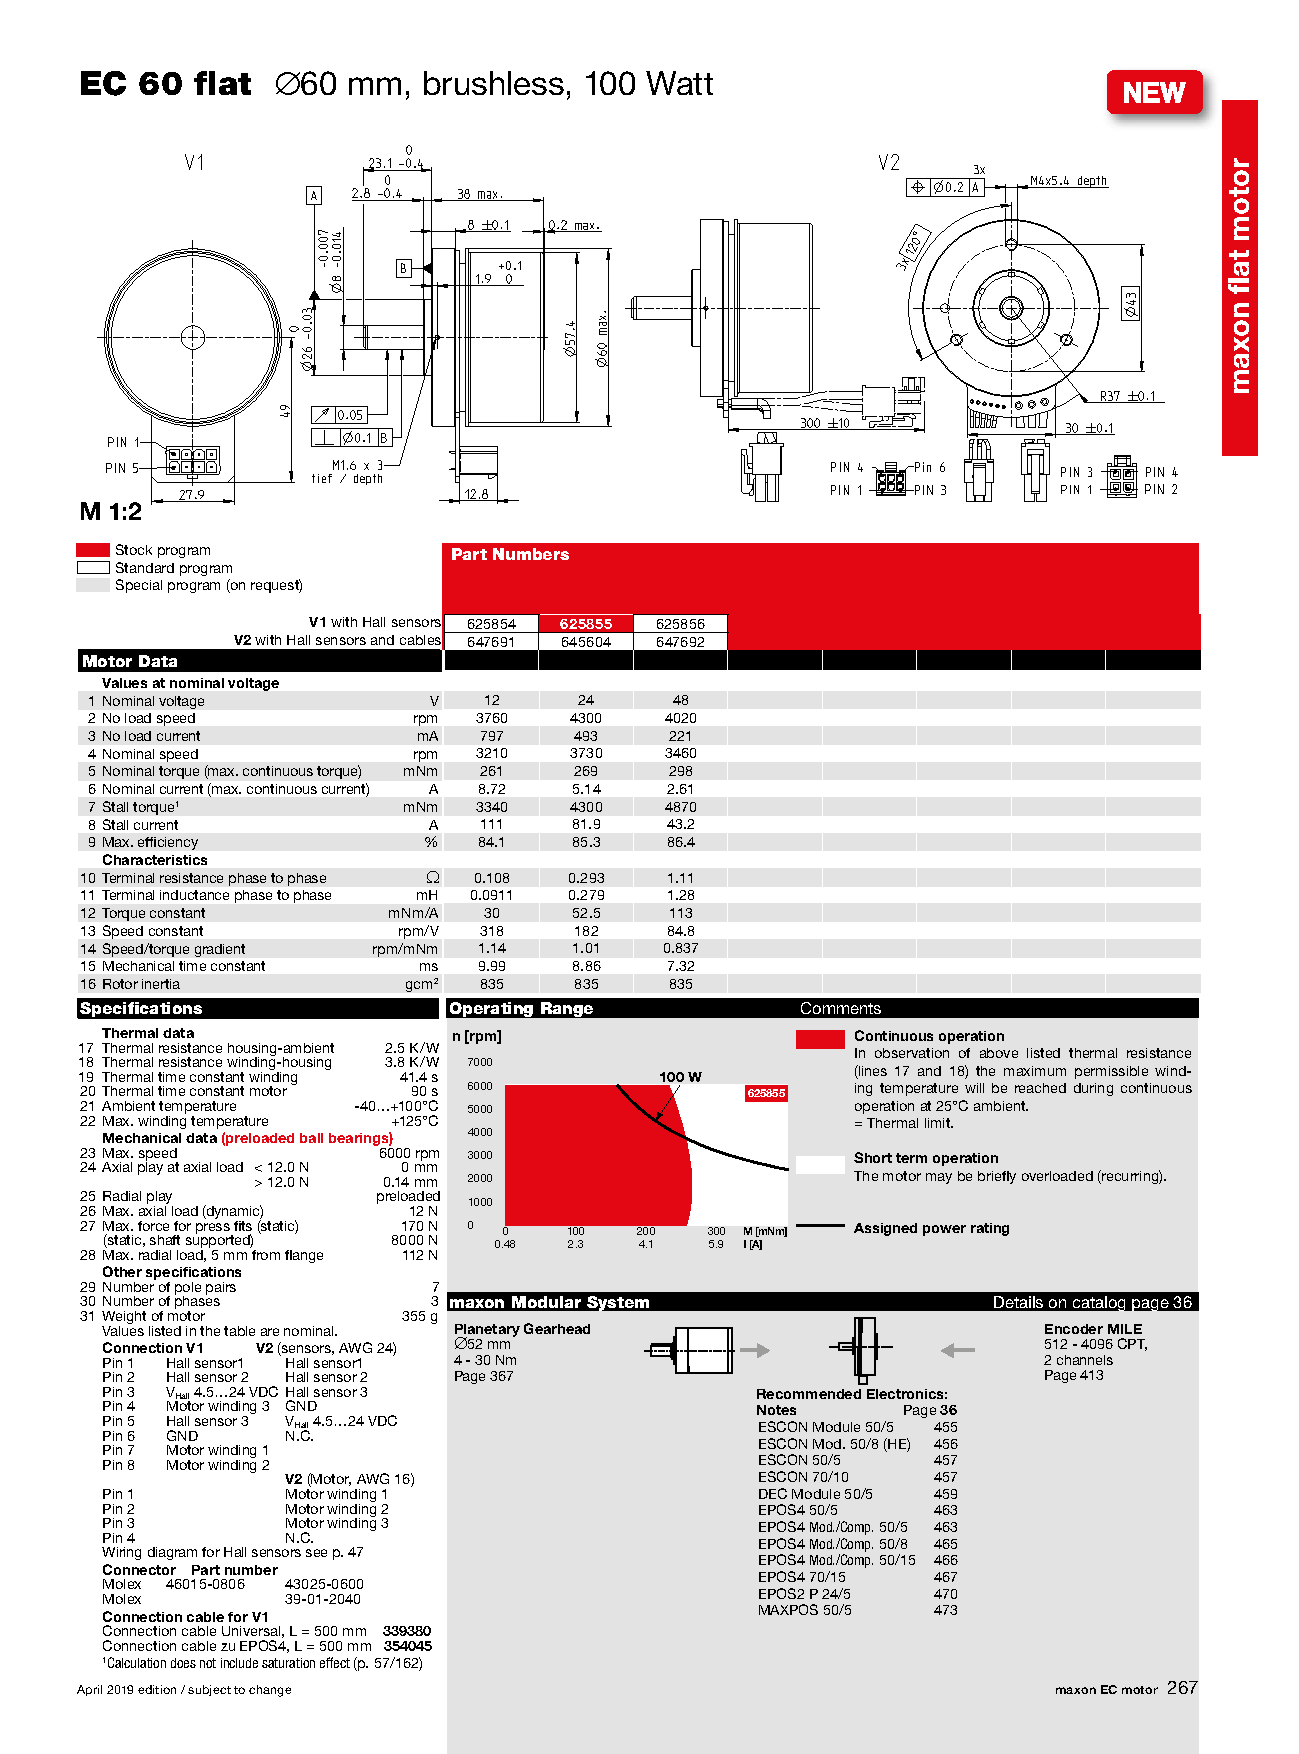
\includepdf[pages=-]{pdf/maxon_ec60_100W}
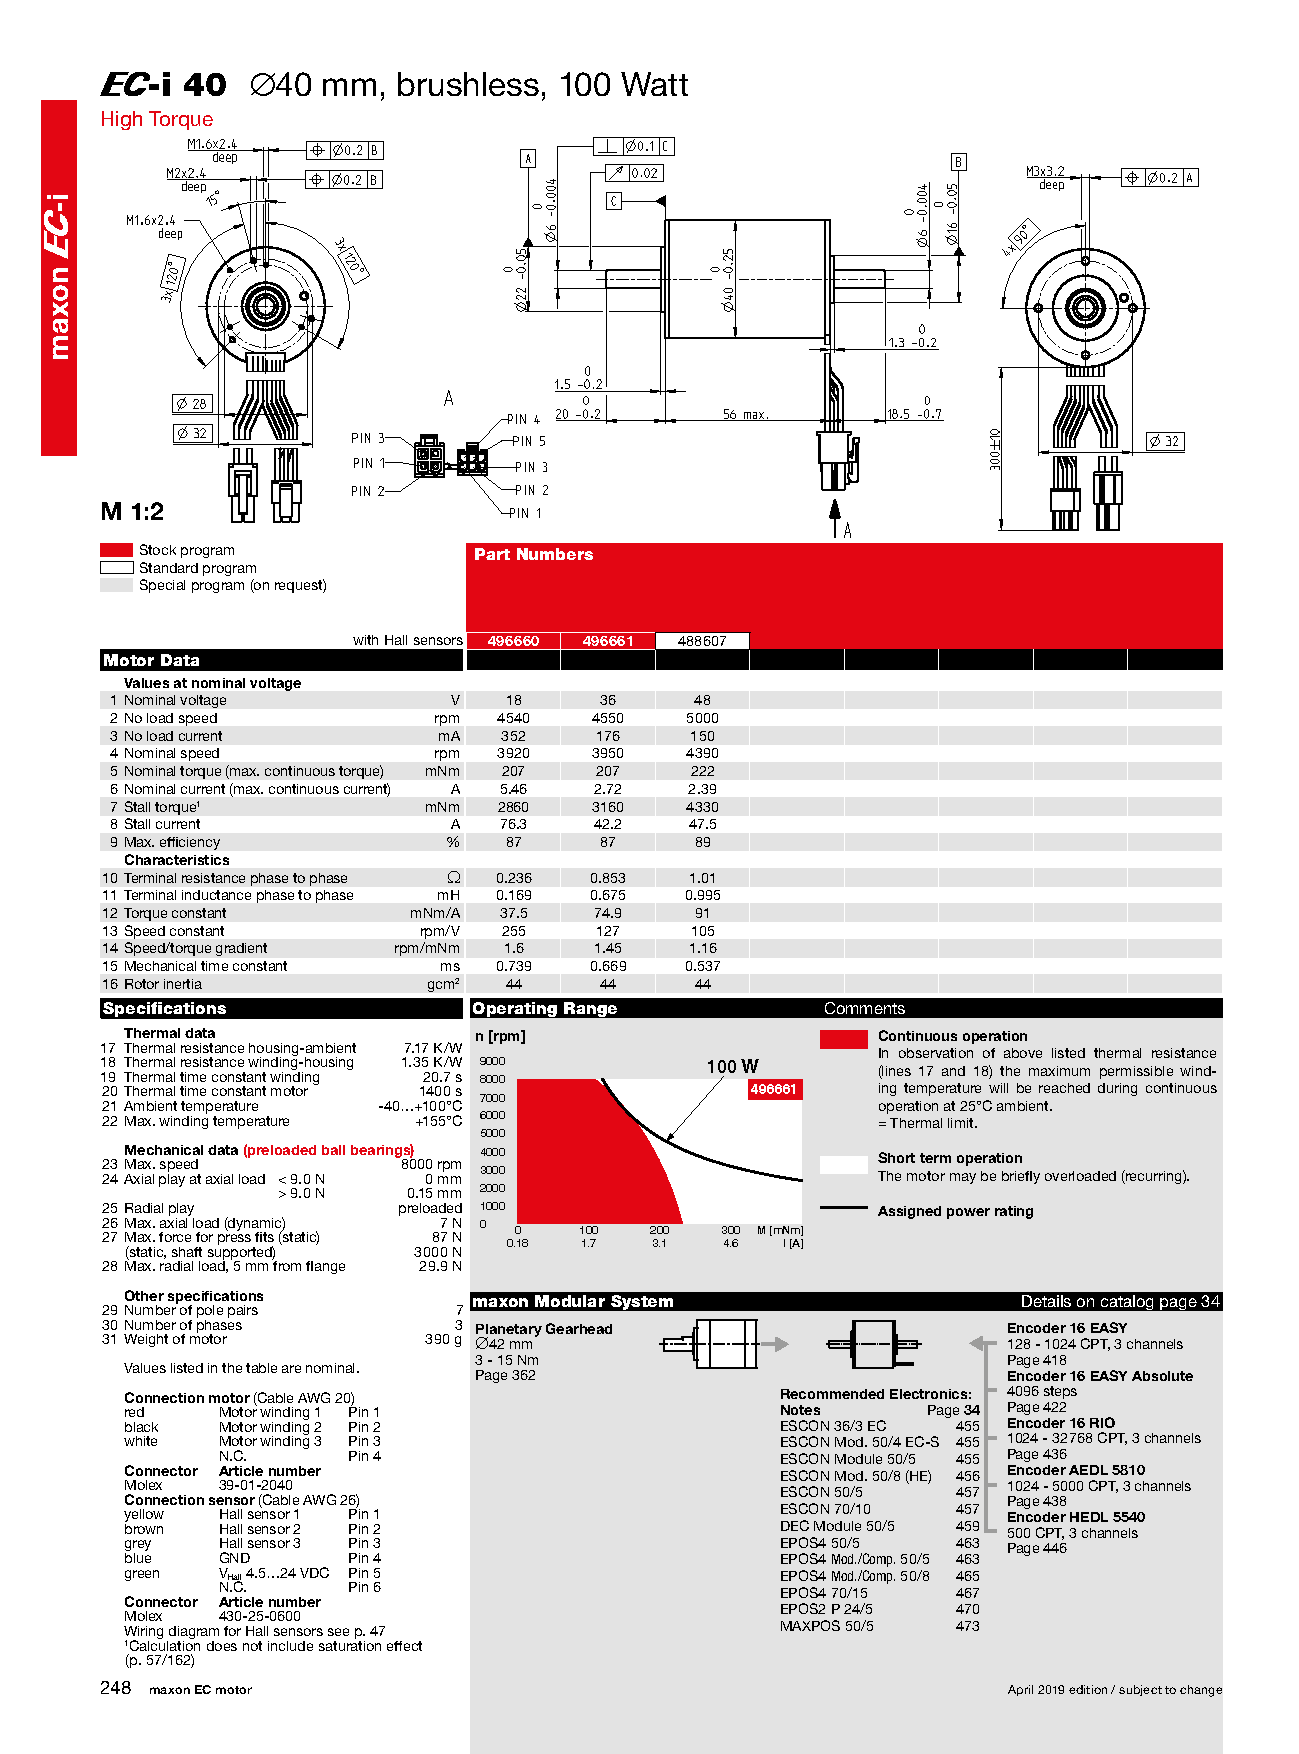
\includepdf[pages=-]{pdf/maxon_eci40_100W}
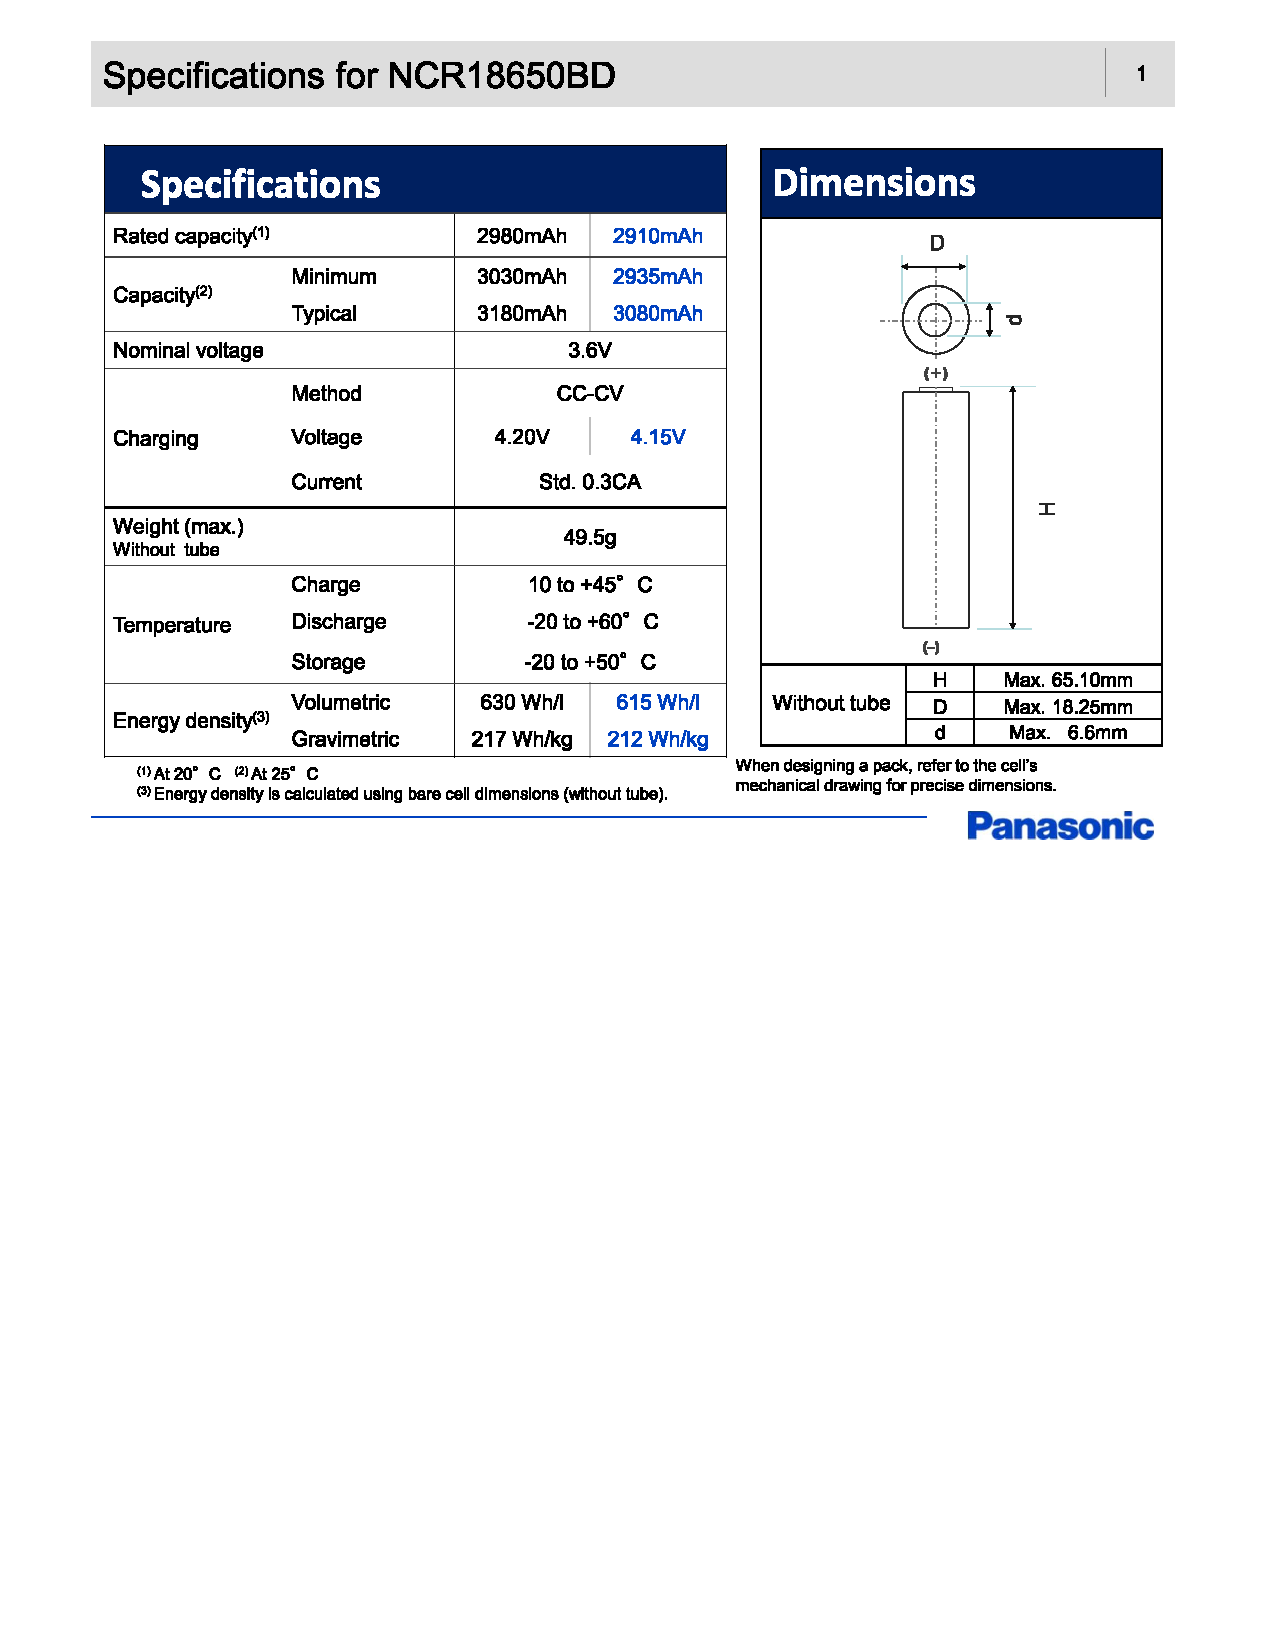
\includepdf[pages=-]{pdf/panasonic_18650}
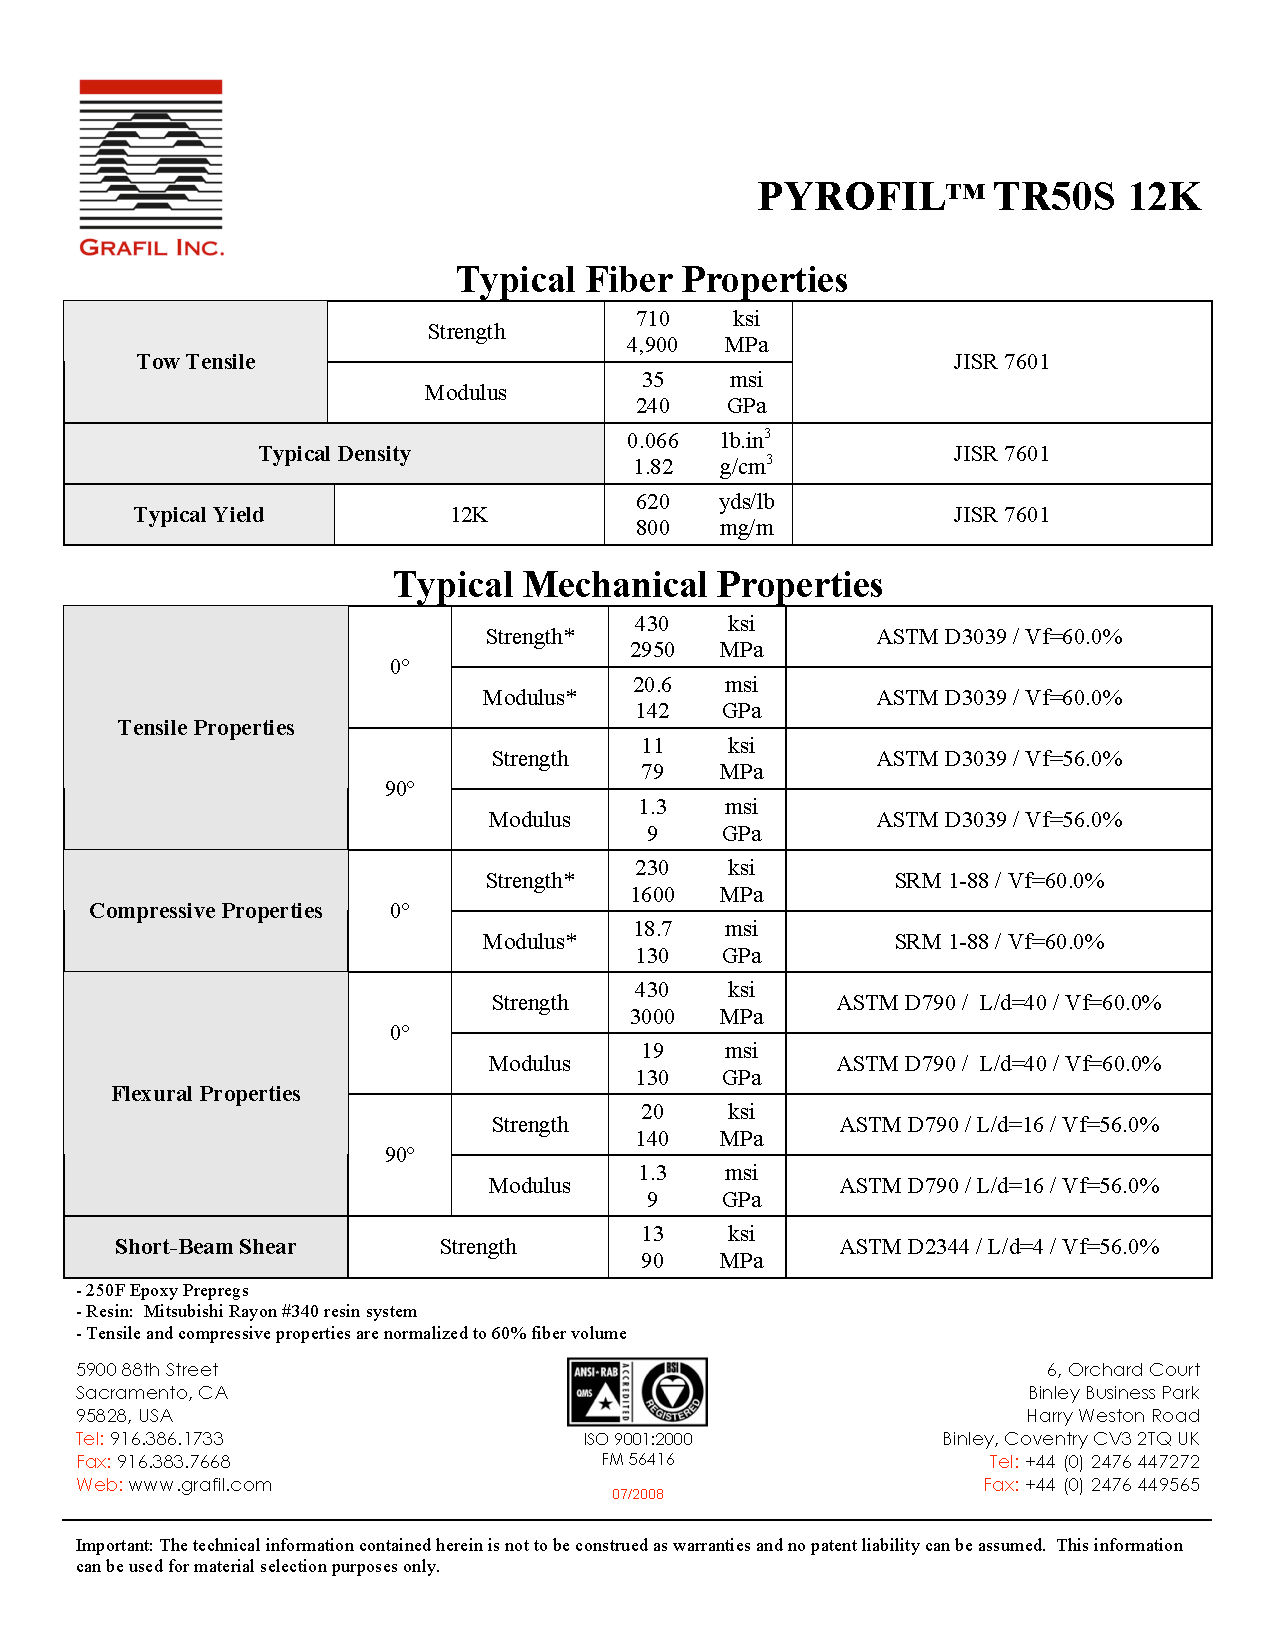
\includepdf[pages=-]{pdf/CarbonFiber}
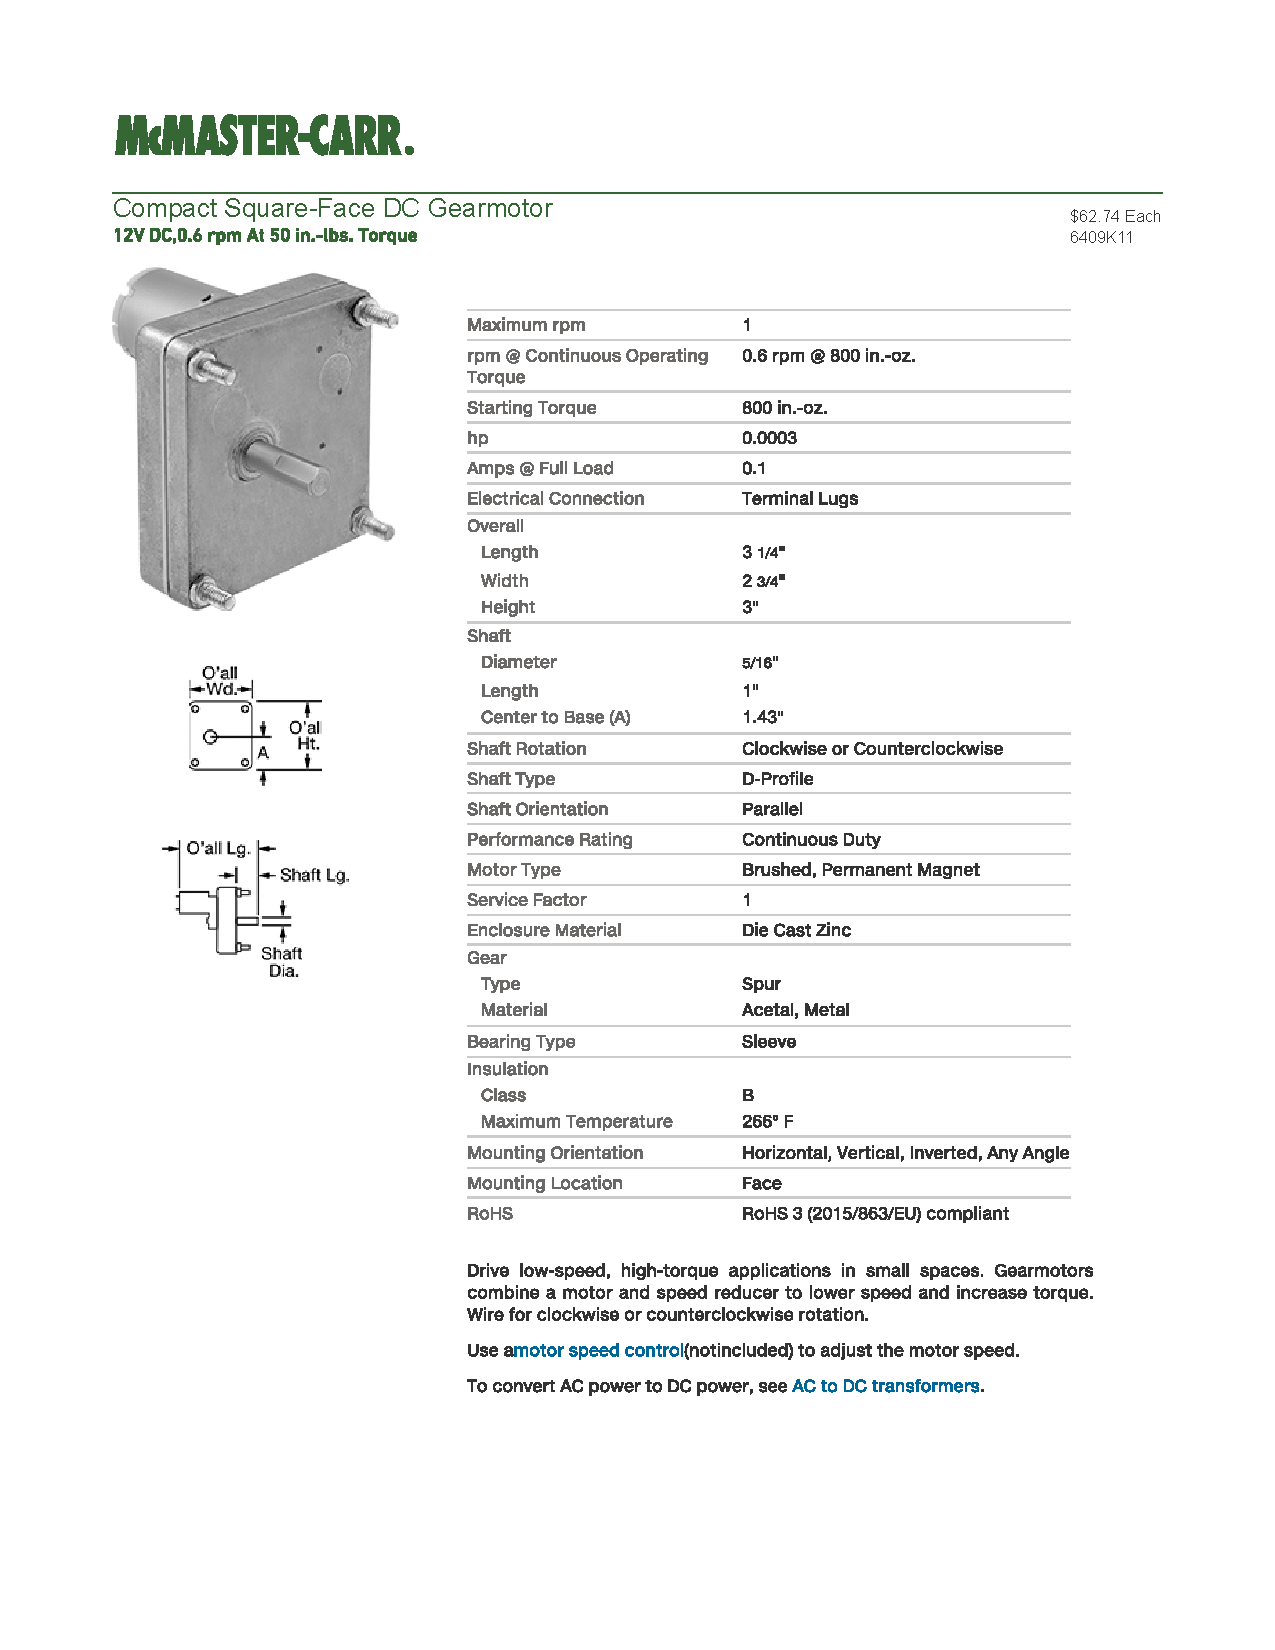
\includepdf[pages=-]{pdf/DCGearMotor}
%\end{comment}